% \documentclass[a4paper, 11pt]{article}
\documentclass{article}

\usepackage[dvipsnames]{xcolor}
\usepackage{ctex}
\usepackage{graphicx}
\usepackage[unicode]{hyperref}
\usepackage{cite}
\usepackage{indentfirst}
\usepackage{listings}
\usepackage{geometry}
\usepackage{amsmath}
\usepackage{tabularx}

\geometry{a4paper, left=2cm, right=2cm, top=1cm, bottom=1.5cm}

% \lstset{
%   language=C++,
%   basicstyle=\fontsize{8}{5}\ttfamily, % 设置代码字体大小为 12pt
%   breaklines=true, % 自动换行
%   numbers=left,
%   showstringspaces = false
% }

%%%%%% 设置字号 %%%%%% 
\newcommand{\chuhao}{\fontsize{nn42pt}{\baselineskip}\selectfont}
\newcommand{\xiaochuhao}{\fontsize{36pt}{\baselineskip}\selectfont}
\newcommand{\yihao}{\fontsize{28pt}{\baselineskip}\selectfont}
\newcommand{\erhao}{\fontsize{21pt}{\baselineskip}\selectfont}
\newcommand{\xiaoerhao}{\fontsize{18pt}{\baselineskip}\selectfont}
\newcommand{\sanhao}{\fontsize{15.75pt}{\baselineskip}\selectfont}
\newcommand{\sihao}{\fontsize{14pt}{\baselineskip}\selectfont}
\newcommand{\xiaosihao}{\fontsize{12pt}{\baselineskip}\selectfont}
\newcommand{\wuhao}{\fontsize{10.5pt}{\baselineskip}\selectfont}
\newcommand{\xiaowuhao}{\fontsize{9pt}{\baselineskip}\selectfont}
\newcommand{\liuhao}{\fontsize{7.875pt}{\baselineskip}\selectfont}
\newcommand{\qihao}{\fontsize{5.25pt}{\baselineskip}\selectfont}

% %%%% 设置 section 属性 %%%%
% \makeatletter
% \renewcommand\section{\@startsection{section}{1}{\z@}%
% {-1.5ex \@plus -.5ex \@minus -.2ex}%
% {.5ex \@plus .1ex}%
% {\normalfont\sihao\CJKfamily{hei}}}
% \makeatother

 %%%% 设置 subsection 属性 %%%%
% \makeatletter
% \renewcommand\subsection{\@startsection{subsection}{1}{\z@}%
% % {-1.25ex \@plus -.5ex \@minus -.2ex}%
% % {-1ex \@plus -.5ex \@minus -.2ex}%
% {-1ex \@plus -.3ex \@minus -.1ex}%
% {.4ex \@plus .1ex}%
% {\normalfont\xiaosihao\CJKfamily{hei}}}
% \makeatother

% %%%% 设置 subsubsection 属性 %%%%
% \makeatletter
% \renewcommand\subsubsection{\@startsection{subsubsection}{1}{\z@}%
% {-1ex \@plus -.5ex \@minus -.2ex}%
% {.3ex \@plus .1ex}%
% {\normalfont\xiaosihao\CJKfamily{hei}}}
% \makeatother

%%%% 段落首行缩进两个字 %%%%
\makeatletter
\let\@afterindentfalse\@afterindenttrue
\@afterindenttrue
\makeatother
% \setlength{\parindent}{2em}  %中文缩进两个汉字位

%%%% 下面的命令重定义页面边距,使其符合中文刊物习惯 %%%%
% \addtolength{\topmargin}{-54pt}
% \setlength{\oddsidemargin}{0.63cm}  % 3.17cm - 1 inch
% \setlength{\evensidemargin}{\oddsidemargin}
% \setlength{\textwidth}{14.66cm}
% \setlength{\textheight}{24.00cm}    % 24.62

%%%% 下面的命令设置行间距与段落间距 %%%%
\linespread{1.0}
% \setlength{\parskip}{1ex}
\setlength{\parskip}{0.5\baselineskip}

% 在导言区进行样式设置
\lstset{
    language=C++, % 设置语言
 	basicstyle=\ttfamily, % 设置字体族
 	breaklines=true, % 自动换行
 	keywordstyle=\bfseries\color{NavyBlue}, % 设置关键字为粗体,颜色为 NavyBlue
 	morekeywords={PressureSensor, Button, Oled}, % 设置更多的关键字,用逗号分隔
 	emph={self}, % 指定强调词,如果有多个,用逗号隔开
    emphstyle=\bfseries\color{Rhodamine}, % 强调词样式设置
    commentstyle=\itshape\color{black!50!white}, % 设置注释样式,斜体,浅灰色
    stringstyle=\bfseries\color{PineGreen!90!black}, % 设置字符串样式
    columns=flexible,
    numbers=left, % 显示行号在左边
    numbersep=2em, % 设置行号的具体位置
    numberstyle=\footnotesize, % 缩小行号
    % frame=single, % 边框
	tabsize = 4,  %行缩进
    framesep=1em % 设置代码与边框的距离
}

%%%% 正文开始 %%%%
\begin{document}	
		%%%% 定理类环境的定义 %%%%
\newtheorem{example}{例}             % 整体编号
\newtheorem{algorithm}{算法}
\newtheorem{theorem}{定理}[section]  % 按 section 编号
\newtheorem{definition}{定义}
\newtheorem{axiom}{公理}
\newtheorem{property}{性质}
\newtheorem{proposition}{命题}
\newtheorem{lemma}{引理}
\newtheorem{corollary}{推论}
\newtheorem{remark}{注解}
\newtheorem{condition}{条件}
\newtheorem{conclusion}{结论}
\newtheorem{assumption}{假设}

		%%%% 重定义 %%%%
\renewcommand{\contentsname}{目录}  % 将Contents改为目录
\renewcommand{\abstractname}{摘要}  % 将Abstract改为摘要
\renewcommand{\refname}{参考文献}   % 将References改为参考文献
\renewcommand{\indexname}{索引}
\renewcommand{\figurename}{图}
\renewcommand{\tablename}{表}
\renewcommand{\appendixname}{附录}
\renewcommand{\algorithm}{算法}	

		%%% 定义标题格式,包括title,author,affiliation,email等 %%%%
\title{智能仓储系统的开发研究}
% \author{XXX\footnote{电子邮件: XXXXXXXXXXXX@zjut.edu.cn 学号: XXXXXXXXXXXX}\\[2ex]
% \xiaosihao 浙江工业大学\\[2ex]}
\author{\xiaosihao 先进计算与机器人研究所}
%\date{}
		
		%%%% 以下部分是正文 %%%%  
\maketitle
		
\tableofcontents
\newpage

\section{第三章: 显示屏}
\begin{figure}[h]
	\centering
	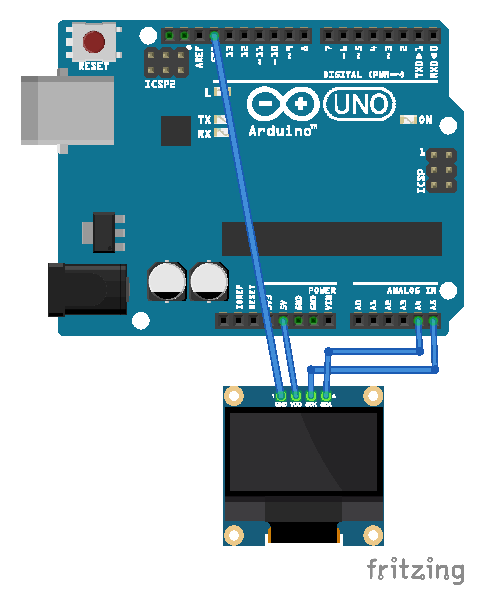
\includegraphics[width=0.6\textwidth]{../Picture/OLED.pdf}
	\caption{显示屏连接}
	\label{fig:显示屏连接}
	\hfill
\end{figure}

\begin{itemize}
	\item 显示器vcc接arduino上的5V;
	\item 显示器Gnd接arduino上的Gnd;
	\item 显示器SCL接arduino上的SCL;
	\item 显示器SDA接arduino上的SDA;
\end{itemize}


\subsection{Oled}
Oled类的核心变量是data1, data2, data3, data4。这是一块显示屏需要显示的内容, 在接下来通信的章节会赋予实际意义。
\begin{lstlisting}
#include <Adafruit_GFX.h>
#include <Adafruit\_SSD1306.h>

class Oled {
private:
  String data1, data2, data3, data4;
  Adafruit\_SSD1306 display;
public:
  Oled();
  void init();
  void Set_Oledvalue(String d1, String d2, String d3, String d4);
  void Output_Oledvalue();
};
\end{lstlisting}

其中Adafruit\_SSD1306是与显示屏相关的类, 在构造函数Oled()中实例化这个类为display。
128,64分别是OLED屏的宽和高, Wire表示用的I2C通信, 没有设置重置引脚时, 就是-1。
\begin{lstlisting}
Oled::Oled() {
  display = Adafruit\_SSD1306(128, 64, &Wire, -1);
};  
\end{lstlisting}

实例化Adafruit\_SSD1306类后, 还不能直接用这个显示屏来显示内容,还需要一步arduino和显示屏的开始通信display.begin。
这一步放在构造函数里, 不能成功显示内容。如果放在loop里调用, 则会出现显示屏内容闪烁的情况。
如果放在setup里调用, 就可以成功稳定显示内容。0x3C为IIC地址。
\begin{lstlisting}
void Oled::init(){
  display.begin(SSD1306_SWITCHCAPVCC, 0x3C);
};  
\end{lstlisting}

Set\_Oledvalue是通过赋值来更新"data"变量,
\begin{lstlisting}
void Oled::Set_Oledvalue(String d1, String d2, String d3, String d4){
  data1 = d1;
  data2 = d2;
  data3 = d3;
  data4 = d4;
};  
\end{lstlisting}

Output\_Oledvalue是将"data"变量在Oled屏上显示。
\begin{lstlisting}
void Oled::Output_Oledvalue(){
  display.clearDisplay(); // 清除屏幕

  //设置字体大小 设置字体颜色,白色可见
  display.setTextSize(2);
  display.setTextColor(WHITE);

  //设置光标位置 
  display.setCursor(5, 5);
  display.print(data1);
  display.setCursor(69, 5);
  display.print(data2);
  display.setCursor(5, 37);
  display.print(data3);
  display.setCursor(69, 37);
  display.print(data4);

  display.display(); 
};
\end{lstlisting}

\subsection{DISPLAY.ino}
\begin{lstlisting}
演示代码将"CC", "100", "10", "1000"在Oled屏显示。
#include "Oled.h"

Oled oled;

void setup() {
  Serial.begin(9600);
  oled.init();
}

void loop() {
  oled.Set_Oledvalue("CC", "100", "10", "1000");
  oled.Output_Oledvalue();
}
\end{lstlisting}

\end{document} 

